\section{Experimental procedure}

    The followoing task had to be done:\\
    \textbf{\ref{task_1}}: Preparation of a radio frequency resonant circuit with the insertion of an iron powde probe in a cryostate\\
    \textbf{\ref{task_2}}: Find the nuclear spin resonance by varying the NMR-pulse frequency while recording a spectrum of the $^{57}$Fe nuclear spin ensemble and calculation of the local magnetic field\\
    \textbf{\ref{task_3}}: Optimization of the pulse sequence by recording a rotation angle curve\\
    \textbf{\ref{task_4}}: Find the spin-spin- and spin-lattice relaxation constants $T_2 \text{ and } T_1$.   

	\subsection{Preparation of a high frequency resonant circuit}
    \label{task_1}
    First one has to prepare a copper coil with a diameter big enough to hold an iron powder assay. After the coil is wrapped one has to sold it onto the contacts of a stick, which provides a mechanism to tune the measured frequency to find the resonance frequency. While solding one has to be careful to make sure, that one do not take to much tin, because the resisteaces of tin and copper are different. In the same way the soldered point should connect the contact and the coil directly, otherwise this could influence the results while tuning to the resonance frequency.
    \begin{center}
           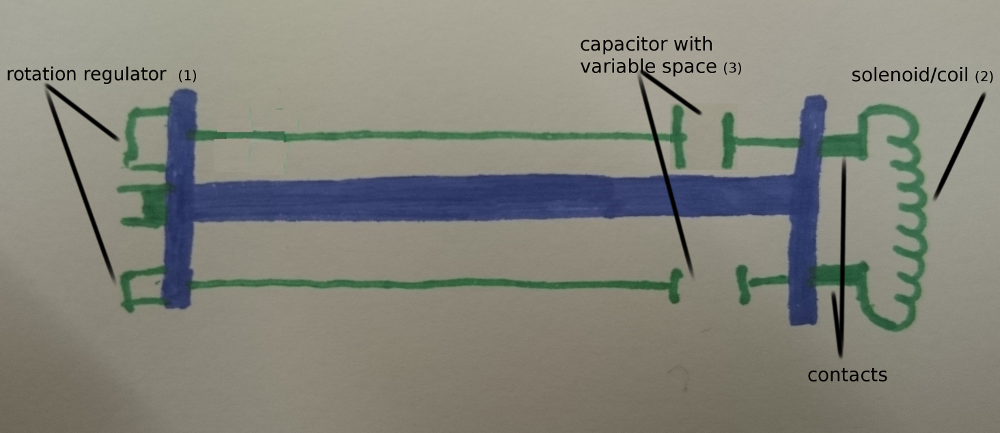
\includegraphics[scale=0.4]{pic/Skizze_Sonde.png} 
           \captionof{figure}{basic sketch of a probe with a coil on it}
           \label{fig:sketch}
    \end{center}
    The rotation regulator (\ref{fig:sketch}.1) varies the space between the capacitor's plates (\ref{fig:sketch}.3) so one can tune the frequency of the solenoid (\ref{fig:sketch}.2).
    \subsection{Finding of the nuclear spin resonance by varying the pulse frequency}
    \label{task_2}
    After the preparation of the solenoid and the insertion of the probe into the cryostat one has to mention what the different paramters, the measurement software has, do with the curve. The different parameters one could vary are $pw$, $\tau$, $rd$ and $ad$. $pw$ makes the magnitude look more gaussian and gives it a bigger value by make the imaginary and real parts more oscillating the higher it is. Varying $\tau$ shows less oscillations and a lower magnitude the higher $\tau$ is. At least one can also vary the parameter $rd$. The higher it is, the more oscillations can be found. One varies this parameters to better fit the magnitude to a gaussian. This means, one searches parameters with a low amount of oscillations, which also have not a big intensity. After the best parameters ($ pw=2\unit{\mu s},\ \tau = 60\unit{\mu s},\ rd = 15\unit{\mu s},\ ad=10\unit{\mu s} $) are found, one looks  at the behavior of the curve at the resonance frequency, a littlebit below and a bit above as shown in the figures \ref{beltd} - \ref{abofs}.
        \begin{figure}[h]
            \subfigure[intensity below resonance frequency in time domain\label{beltd}]{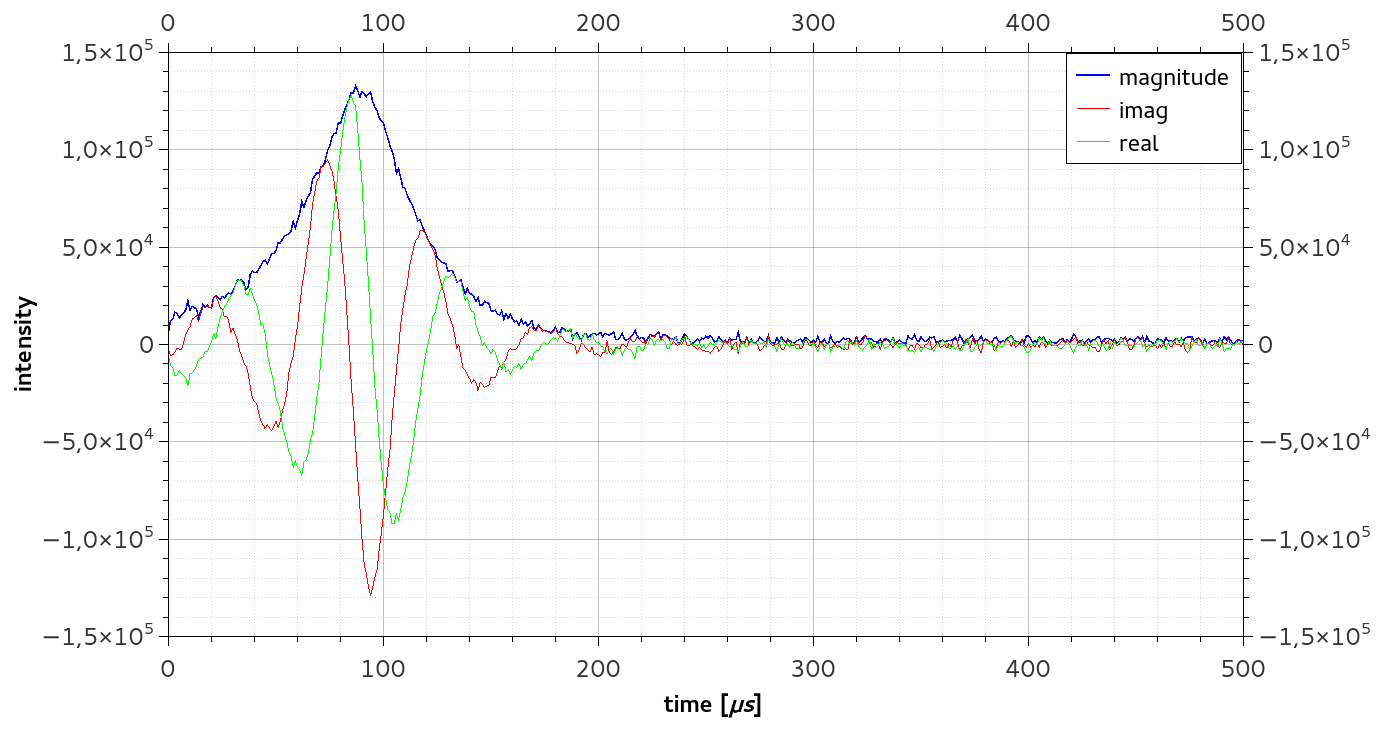
\includegraphics[scale=0.225]{pic/below_resfreq_td.png}}
            \subfigure[intensity below resonance frequency in fourier space\label{belfs}]{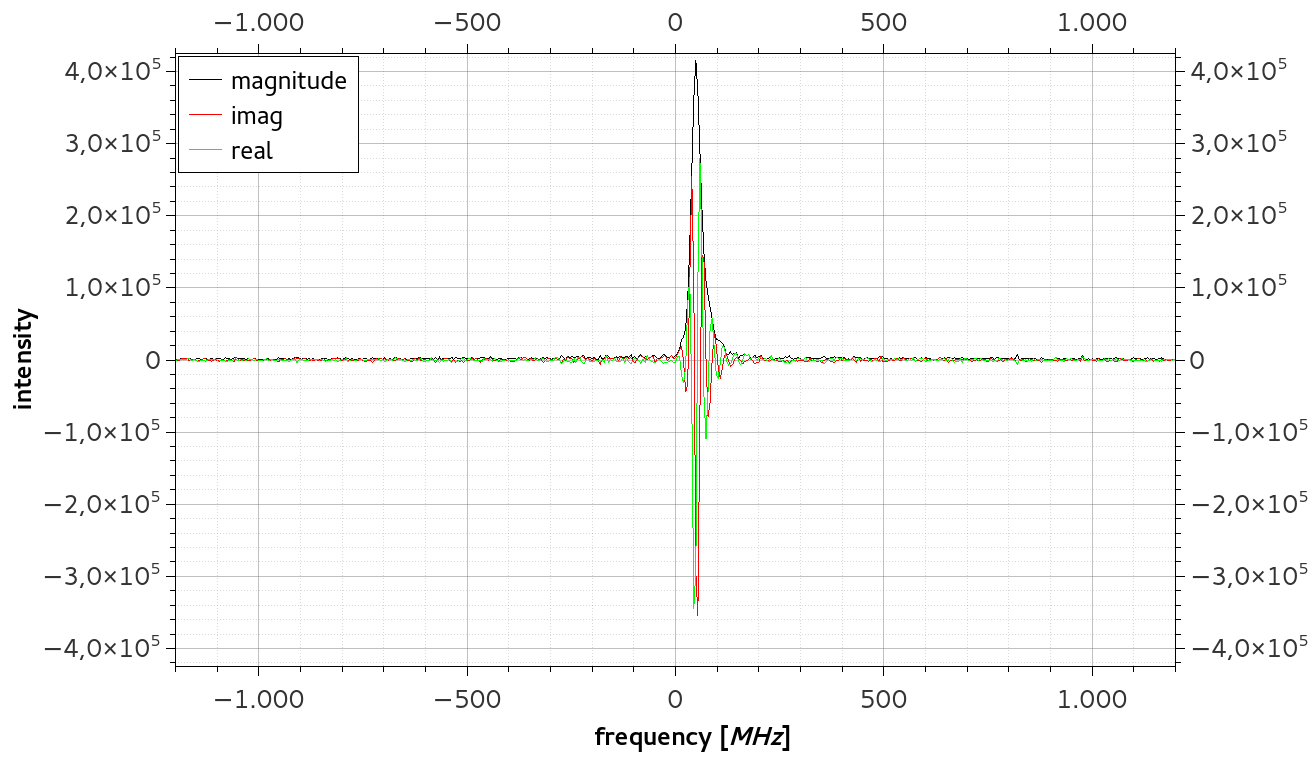
\includegraphics[scale=0.225]{pic/below_resfreq_fs.png}}
            \subfigure[intensity at resonance frequency in time domain\label{restd}]{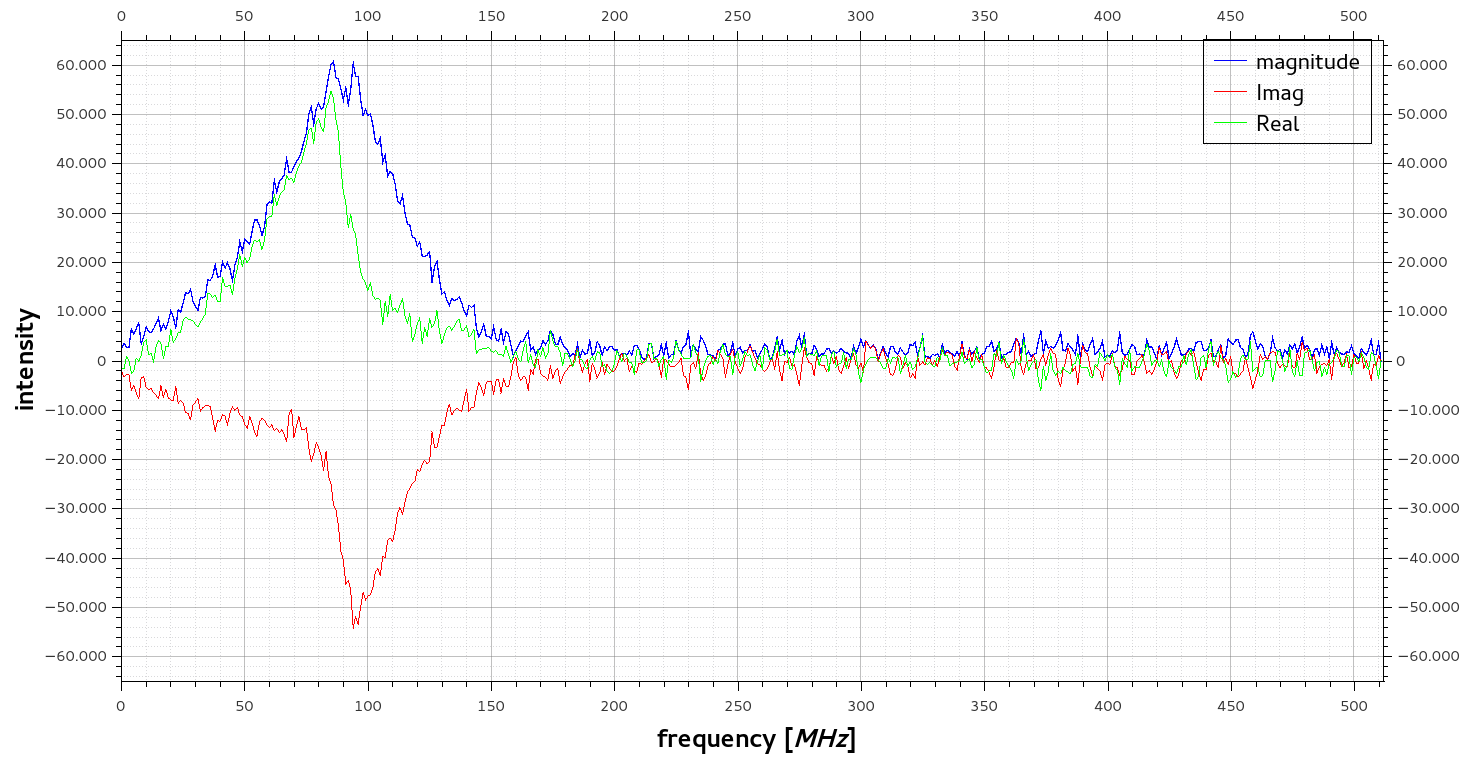
\includegraphics[scale=0.21]{pic/resfreq_td.png}}
            \subfigure[intensity at resonance frequency in fourier space\label{resfs}]{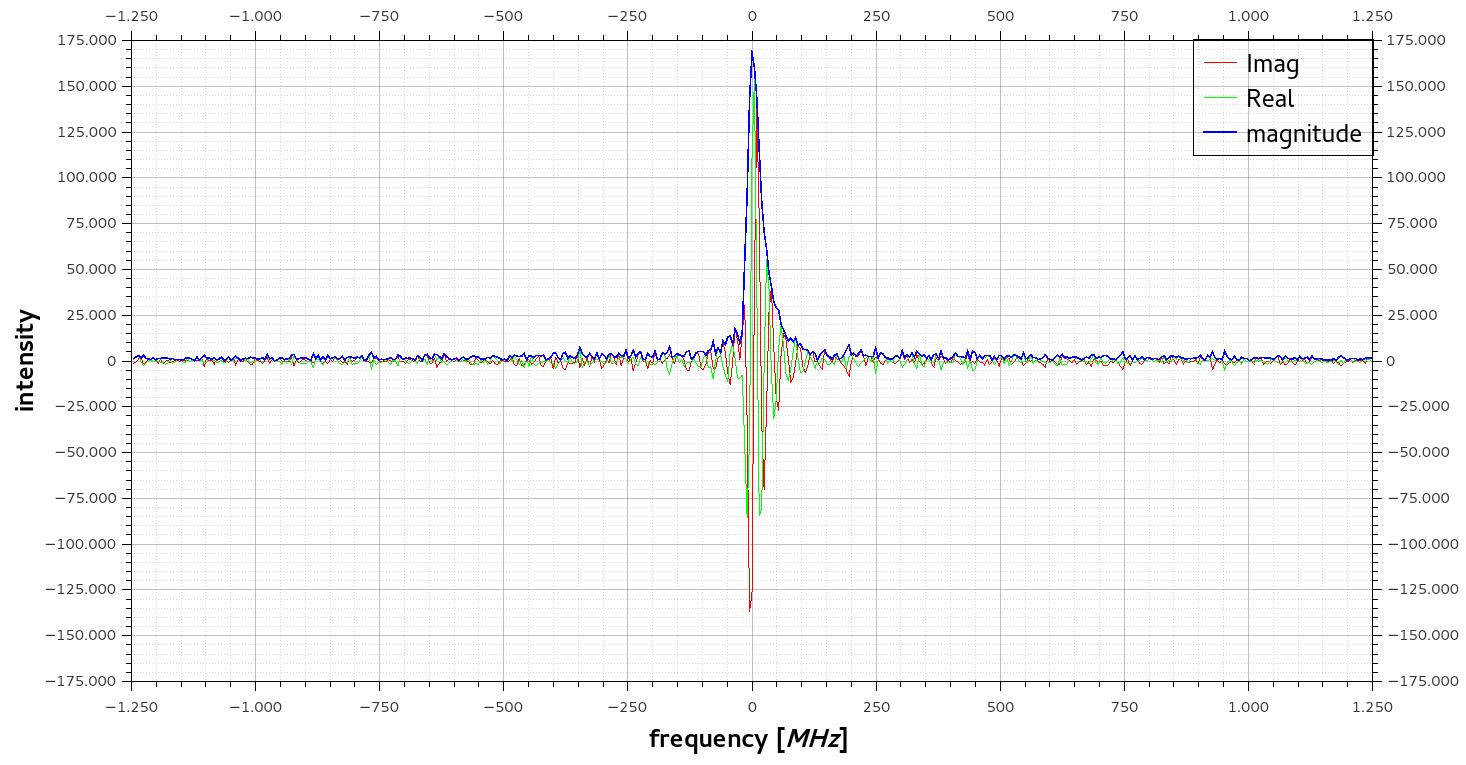
\includegraphics[scale=0.21]{pic/resfreq_fd.png}}
            \subfigure[intensity below resonance frequency in time domain\label{abotd}]{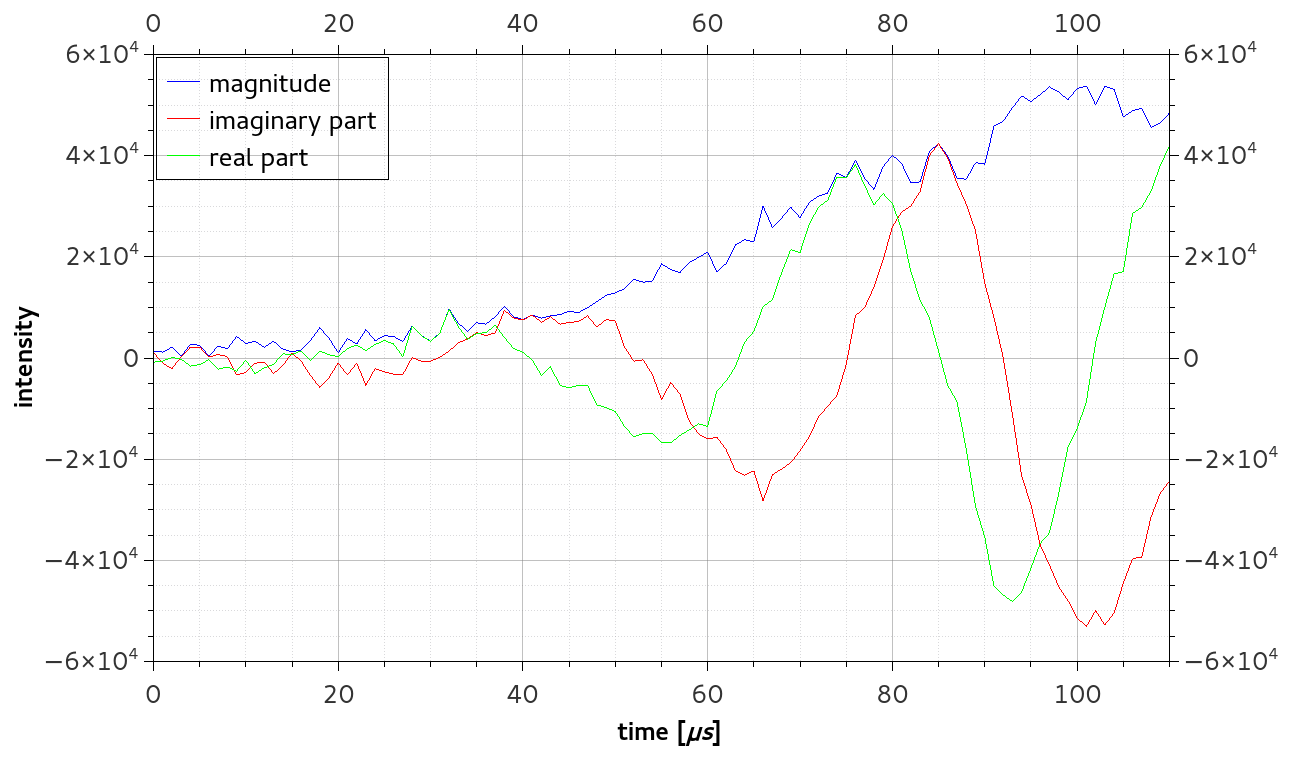
\includegraphics[scale=0.24]{pic/above_resfreq_td.png}}
            \subfigure[intensity below resonance frequency in fourier space\label{abofs}]{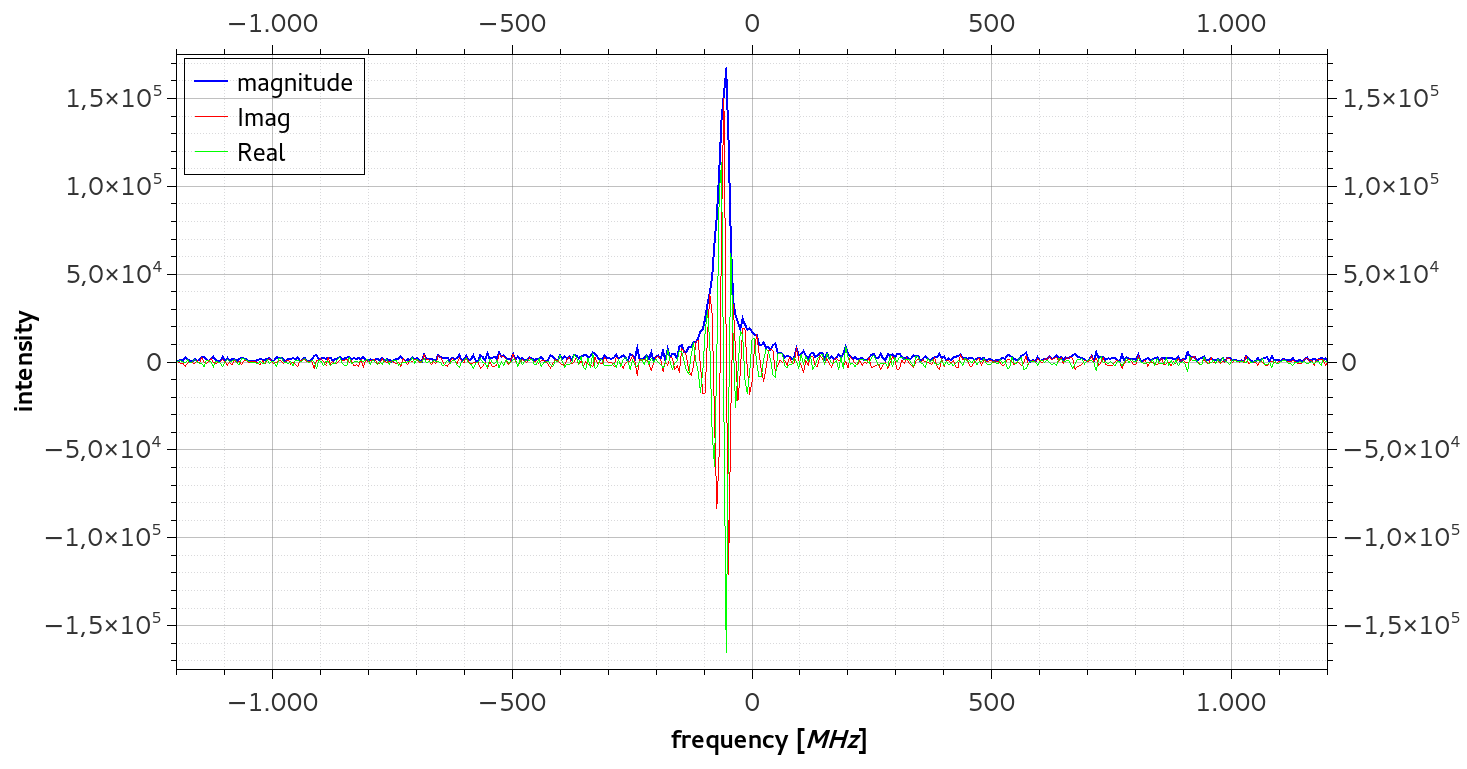
\includegraphics[scale=0.225]{pic/above_resfreq_fs.png}}
            \caption{Different spectra below, at and above the resonance frequency}
         \end{figure}
     One can see that the number of oscillations in \ref{abotd} and \ref{beltd} is bigger than in \ref{restd}. In figure \ref{resfs} one recognizes a good gaussian peak.
     With that information the frequency is found at $\omega_L = 45.47\unit{MHz}$ With the help of the $\gamma$-factor defined in (\ref{eq:gamma}) and the formula (\ref{eq:lamor}), one can calculate the magnetic field as $B_z = \omega_L/\gamma = 0.525\unit{T}$.
         
    \subsection{Optimization of the pulse sequence by recording a rotation angle curve}
    \label{task_3}
    Now one can configure the time intevalls how long the measurement device should wait until it takes a measurement. In both cases, the spin-spin- and the spin-lattice-relaxation one get different times for $\tau$ aus one can see in the diagrams.
    After this measurements the computer takes all magnitude maxima as data points one can analyze.
           \begin{figure}[h]
               \centering
               \subfigure[another test\label{T2}]{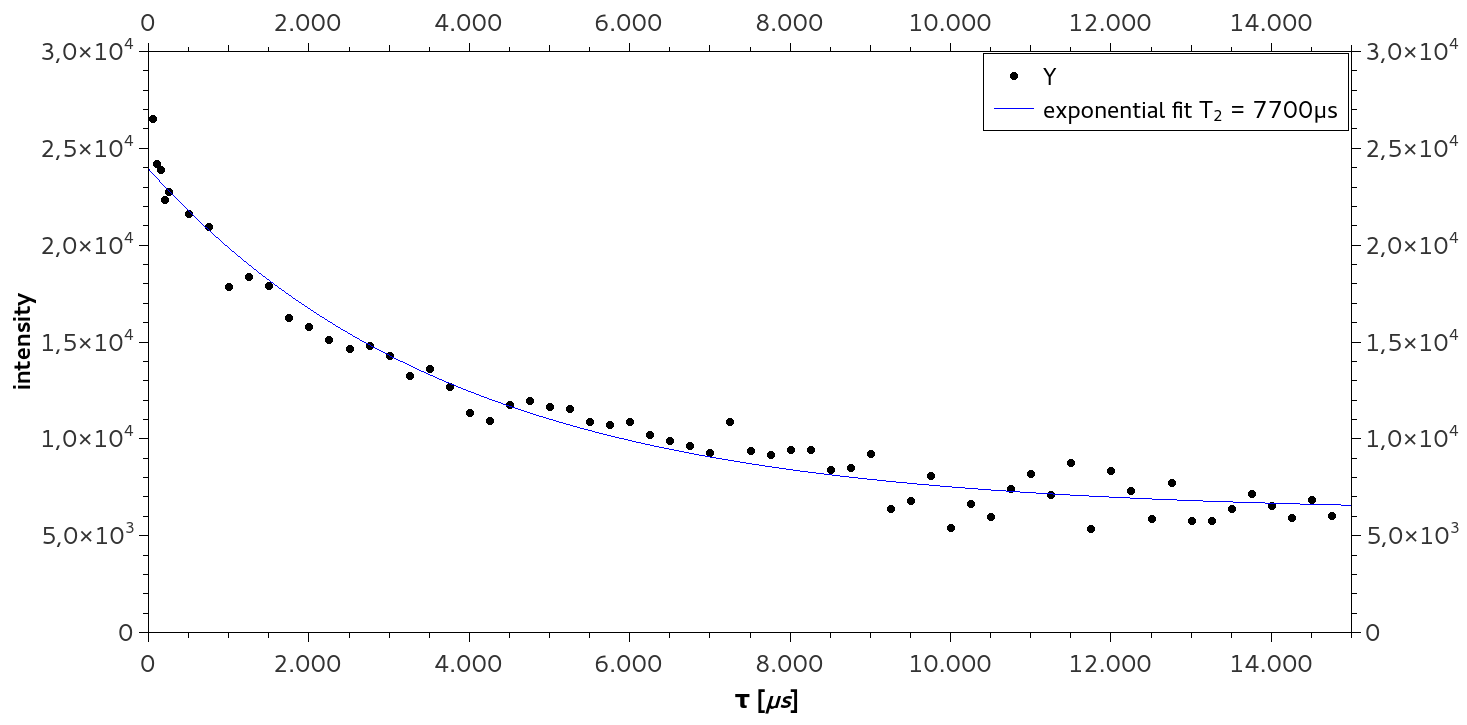
\includegraphics[scale=0.2]{pic/T2.png}}
               \subfigure[some test\label{T1}]{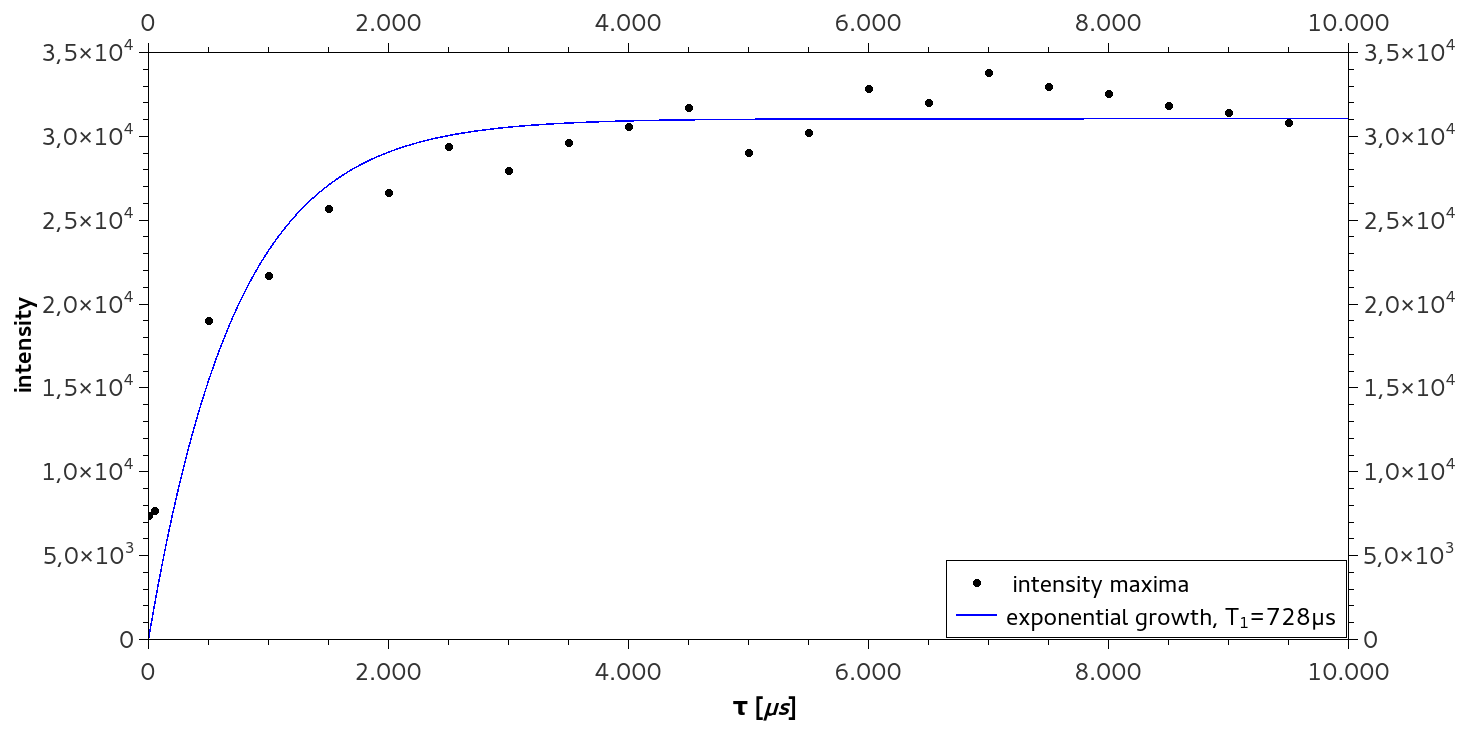
\includegraphics[scale=0.2]{pic/T1.png}}       
               \caption{rotation angle curves for spin-spin- (a) and spin-lattice-relaxation (b) }     
           \end{figure}
    One can recognize that \ref{T1} looks like an exponential growth and \ref{T2} looks similar to an exponential decay. To determine the relaxation constants one uses this information to make fits.        
    \subsection{Determination of the relaxation constants $T_1$ and $T_2$}
    The following fit functions are used;
    \begin{gather}
        y(\tau) = A\cdot(1-e^{-\tau/T_1})\label{fit_T1}\\
        y(\tau) = y_0 + Ae^{-2\tau/T_2}\label{fit_T2}
    \end{gather}
    With a tool called Qtiplot one makes a fit with these funktions a gets the blue line in \ref{T1} and \ref{T2}. The parameters for \ref{fit_T2} are: $$A = 17720,\ y_0 = 6220$ and the spin-spin-relaxation constant $T_2 = 7628\unit{\mu s}$$
    The parameters for the spin-lattice-relaxation are:
    $$ A = 31050,\ T_1 = 728\unit{\mu s} $$
    
    \label{task_4}
    In 
